\chapter{Analyse}\label{ch:analyse}
Dette afsnit viser analyserne, der er blevet i lavet over de forskellige signaler. Der er for alle signaler lavet 4 forskellige plot: Det originale signal, Det Disket Fourrier Transformerede signal, Det Disket Fourrier Transformerede signal med et hanning vindue og Det udglattet Disket Fourrier Transformerede signal.


\section{Motor}
Dette signal er fra motoren på en motorcykel. Man kan se det originale lydsignal på figur \ref{fig:Motor original}.
\begin{figure}[H]
	\centering
	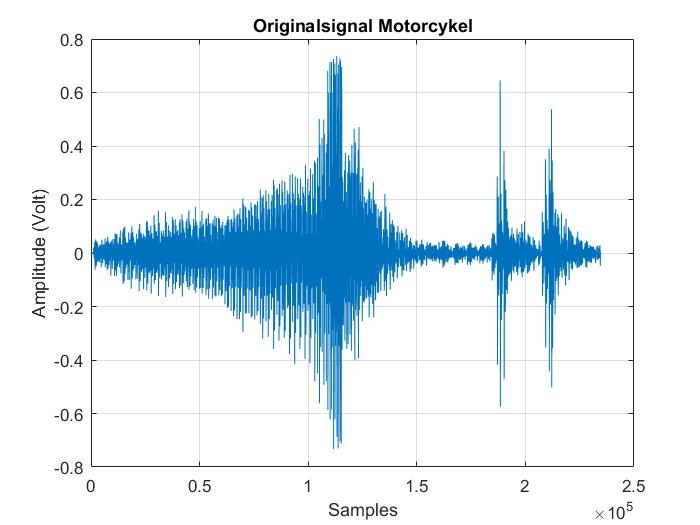
\includegraphics[width=120mm]{figures/Motor/original.jpg}
	\caption{DFT Det originale signal fra en Motor}
	\label{fig:Motor original}
\end{figure}

Det originale signal er blevet fast fourrier transformeret og er blevet plottet på en logoritmisk skala på figur \ref{fig:Motor DFT}. Det i øjenfaldende på dette plot er, at signalet indeholder mange forholdsvis lave toner og  mange forskellige frekvenser. Det kan desuden ses at signalet laver et drop ved omkring 10kHz. Dette ligner rigtig meget et spor fra en tidligere samplingsfrekvens fra samme signal. Dette betyder derfor også, at alle værdier efter dette drop ikke kan bruges til noget analysemæssigt.

\begin{figure}[H]
	\centering
	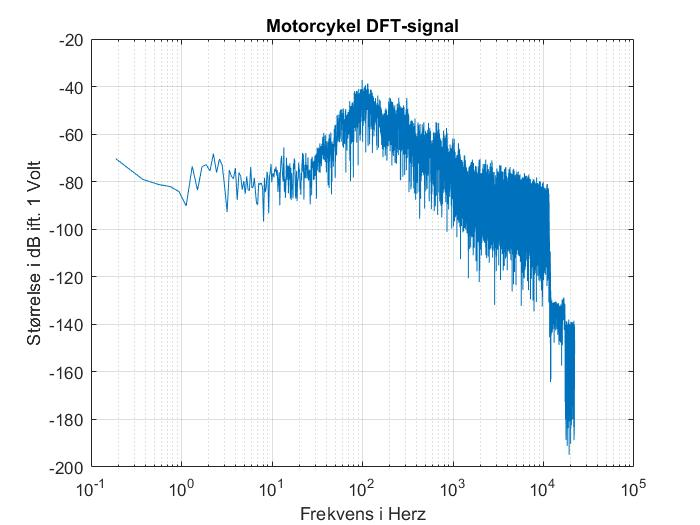
\includegraphics[width=120mm]{figures/Motor/DFT.jpg}
	\caption{DFT Analyse af et signal fra en Motor}
	\label{fig:Motor DFT}
\end{figure}

Det DFT-transfomerede signal er blevet vægtet ved brug af et hanningvindue. Resultatet ses på figur \ref{fig:Motor hanning}. Som man kan se på figuren er der ikke det helt store at hente ved hanningviduet på denne funktion. Dette har været gennemgående for alle funktionerne, at Hanning-vinduet eller en anden vindues-funktion ikke havde nogen stor indvirkning. Derfor er der heller ikke vist figurer med resultatet efter vægtningen med et hanningvindue af resten af signalerne.
\begin{figure}[H]
	\centering
	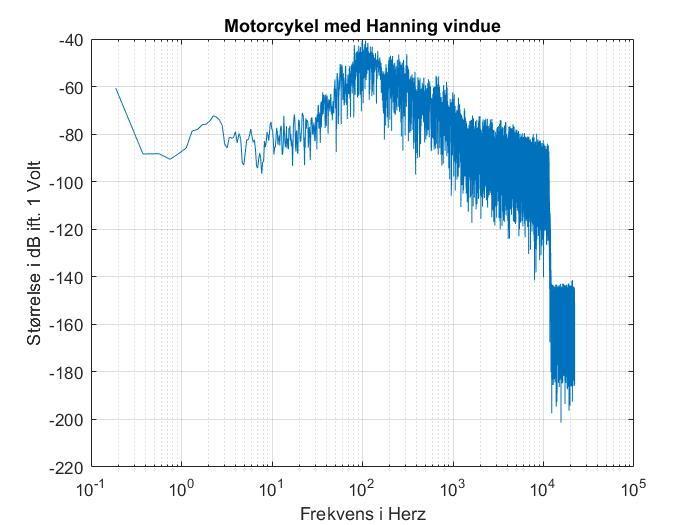
\includegraphics[width=120mm]{figures/Motor/hanning.jpg}
	\caption{DFT Analyse af et signal fra en Motor med et hanningvindue}
	\label{fig:Motor hanning}
\end{figure}

\begin{figure}[H]
	\centering
	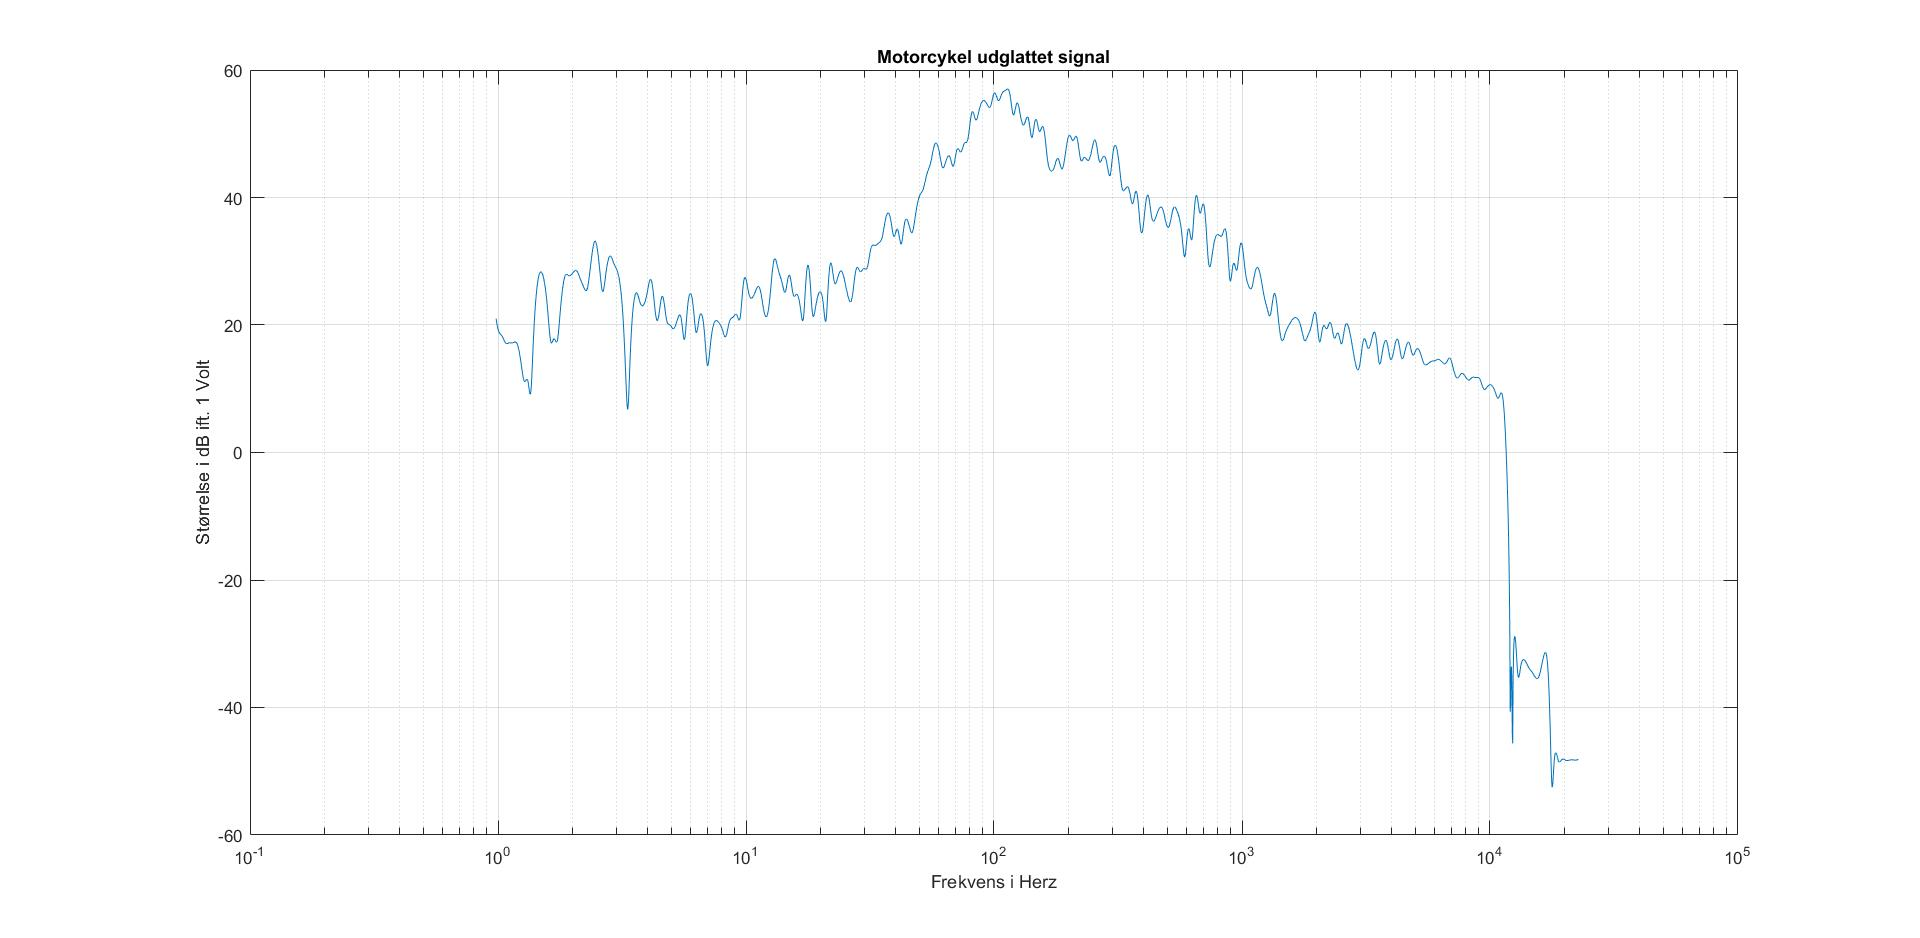
\includegraphics[width=140mm]{figures/Motor/udglattet.jpg}
	\caption{Det udglattede DFT signal fra en Motor}
	\label{fig:Motor udglattet}
\end{figure}
\newpage
\section{Klaver}
Dette signal er fra et klaver. Man kan se det originale lydsignal på figur \ref{fig:Klaver original}.
\begin{figure}[H]
	\centering
	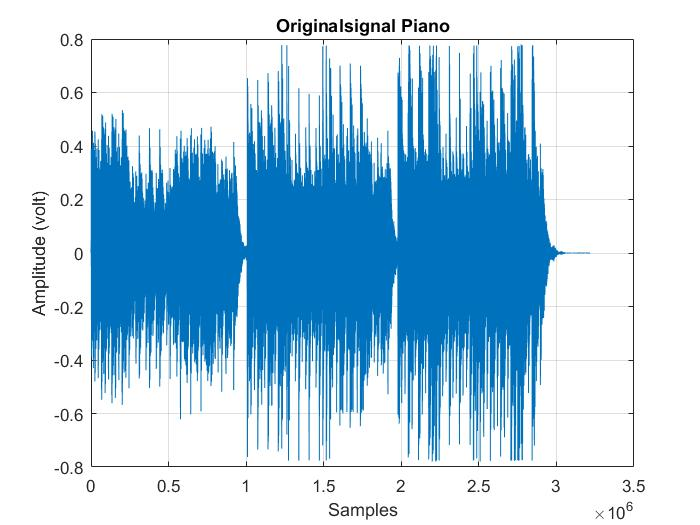
\includegraphics[width=140mm]{figures/Piano/original.jpg}
	\caption{DFT Det originale signal fra et klaver}
	\label{fig:Klaver original}
\end{figure}

Det originale signal er blevet fast fourrier transformeret og er blevet plottet på en logoritmisk skala på figur \ref{fig:Klaver DFT}. Det i øjenfaldende på dette plot er, at det indeholder stor energi omkring 100Hz-1000Hz og indeholder mange præcise unikke frekvenser i dette område. Dette giver også rigtig god mening idet, klaveret spiller mange af de dybe toner på lydfilen.
\begin{figure}[H]
	\centering
	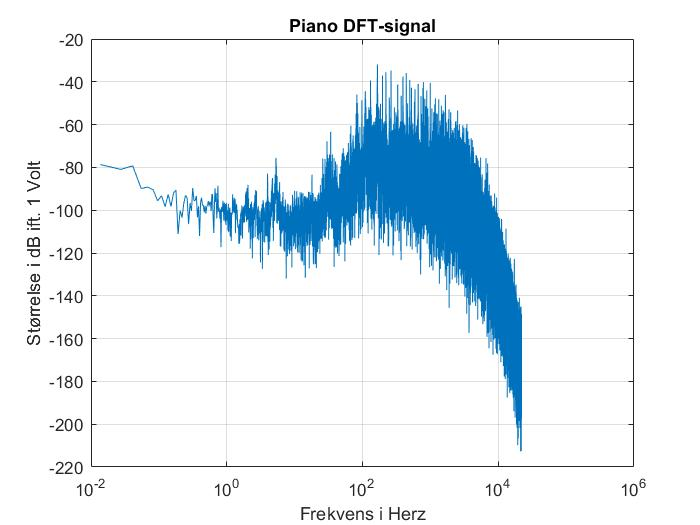
\includegraphics[width=110mm]{figures/Piano/DFT.jpg}
	\caption{DFT Analyse af et signal fra et Klaver}
	\label{fig:Klaver DFT}
\end{figure}

\begin{figure}[H]
	\centering
	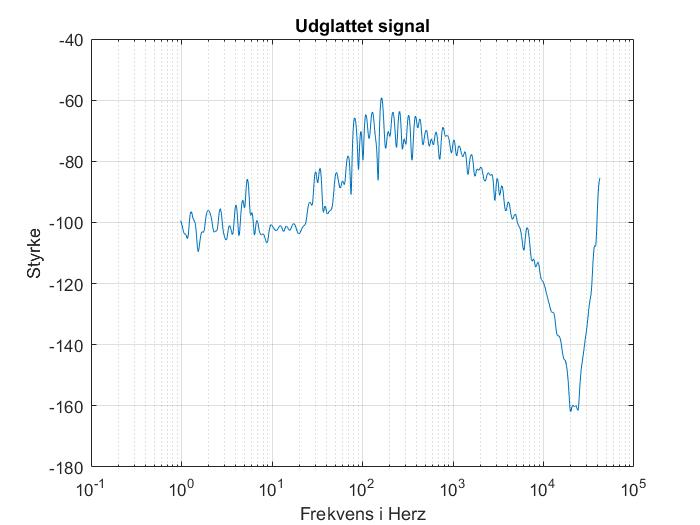
\includegraphics[width=120mm]{figures/Piano/udglattet.jpg}
	\caption{Det udglattede DFT signal fra et Klaver}
	\label{fig:Klaver udglattet}
\end{figure}
\newpage

\section{Symfoni}
Dette signal er fra et symfoniorkester. Man kan se det originale lydsignal på figur \ref{fig:Symfoni original}.
\begin{figure}[H]
	\centering
	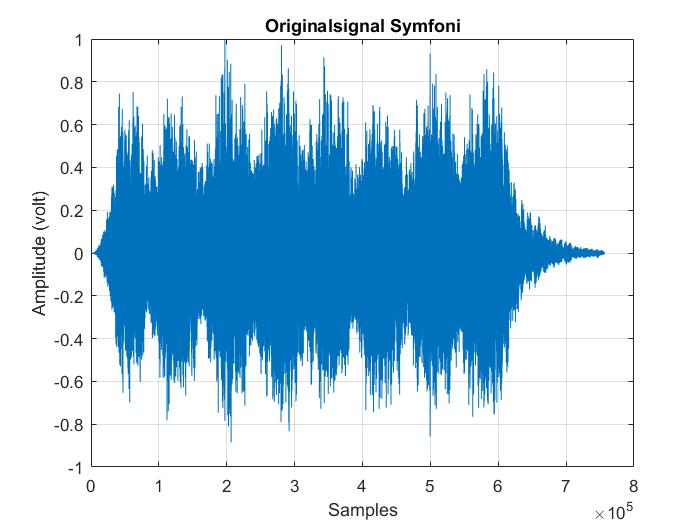
\includegraphics[width=140mm]{figures/Symfoni/original.jpg}
	\caption{DFT Det originale signal fra en Symfoni}
	\label{fig:Symfoni original}
\end{figure}

Det originale signal er blevet fast fourrier transformeret og er blevet plottet på en logoritmisk skala på figur \ref{fig:Symfoni DFT}. Det i øjenfaldende på dette plot er, at det indeholder mange forskellige frekvenser fra de forskellige instrumenter i området 100Hz-1000Hz.
\begin{figure}[H]
	\centering
	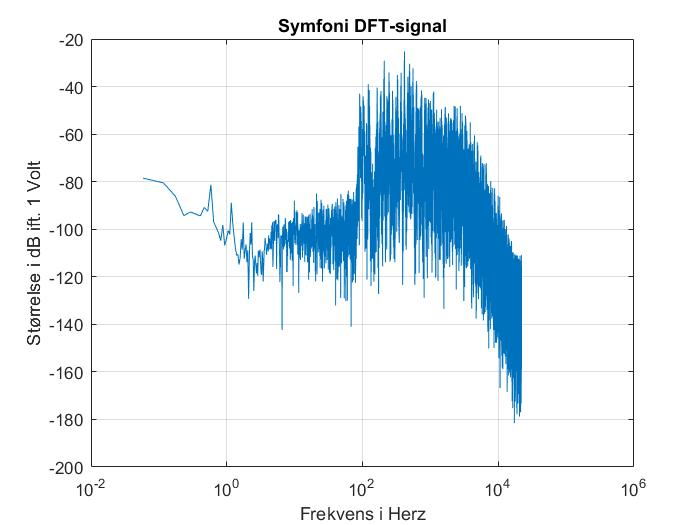
\includegraphics[width=120mm]{figures/Symfoni/DFT.jpg}
	\caption{DFT Analyse af et signal fra en Symfoni}
	\label{fig:Symfoni DFT}
\end{figure}

\begin{figure}[H]
	\centering
	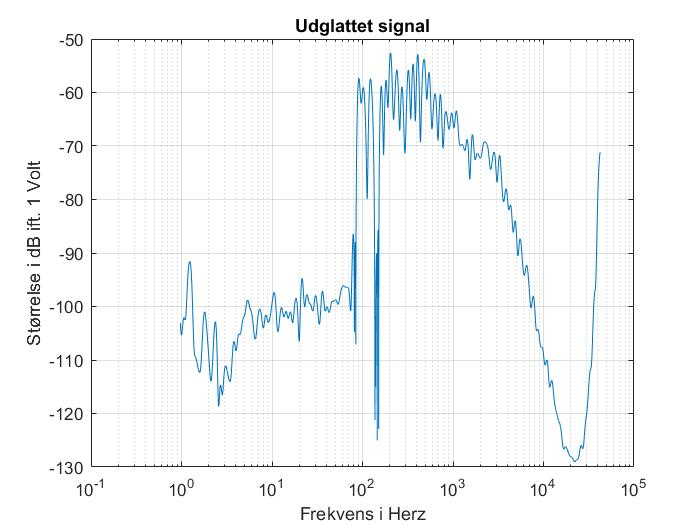
\includegraphics[width=120mm]{figures/Symfoni/udglattet.jpg}
	\caption{Det udglattede DFT signal fra en Symfoni}
	\label{fig:Symfoni udglattet}
\end{figure}

\section{Bass}
Dette signal er fra en bas. Man kan se det originale lydsignal på figur \ref{fig:Bas original}.
\begin{figure}[H]
	\centering
	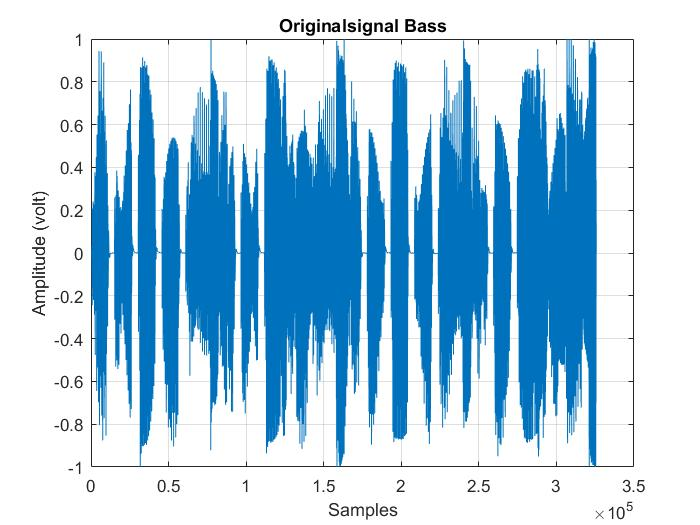
\includegraphics[width=140mm]{figures/Bass/original.jpg}
	\caption{DFT Det originale signal fra en Bas}
	\label{fig:Bas original}
\end{figure}

Det originale signal er blevet fast fourier transformeret og er blevet plottet på en logoritmisk skala på figur \ref{fig:Bas DFT}. Det i øjenfaldende på dette plot er, at frekvenserne fra bassen er rimelig lave i forhold til både klaveret og symfoni-orkesteret. Signalet har også færre frekvenser, "der stikker ud fra mængden", hviket skyldes, at det er en el-bas.

\begin{figure}[H]
	\centering
	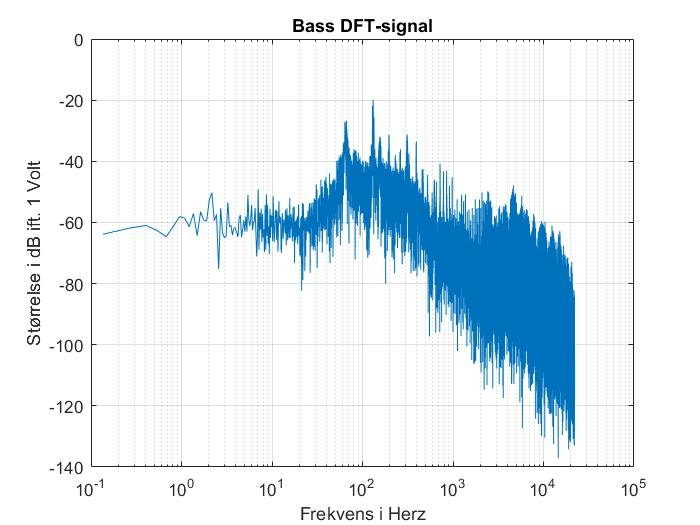
\includegraphics[width=120mm]{figures/Bass/DFT.jpg}
	\caption{DFT Analyse af et signal fra en Bas}
	\label{fig:Bas DFT}
\end{figure}

\begin{figure}[H]
	\centering
	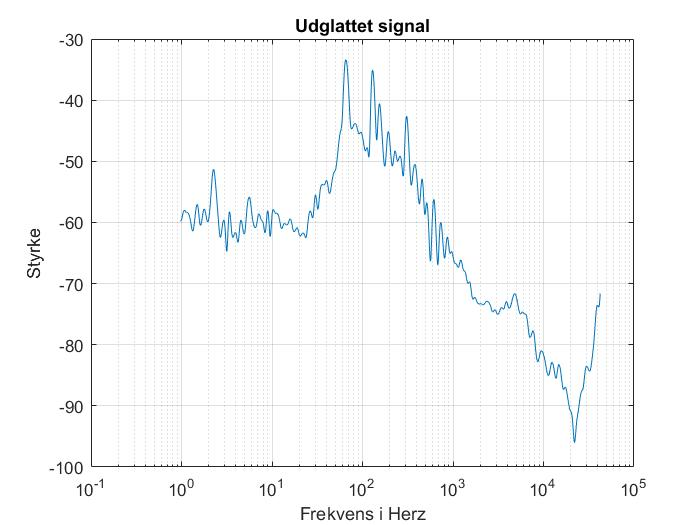
\includegraphics[width=120mm]{figures/Bass/udglattet.jpg}
	\caption{Det udglattede DFT signal fra en Bas}
	\label{fig:Bas udglattet}
\end{figure}



\section{Vinglas}
Dette signal er af en, der knipser på et vinglas. Man kan se det originale lydsignal på figur \ref{fig:Vinglas original}.
\begin{figure}[H]
	\centering
	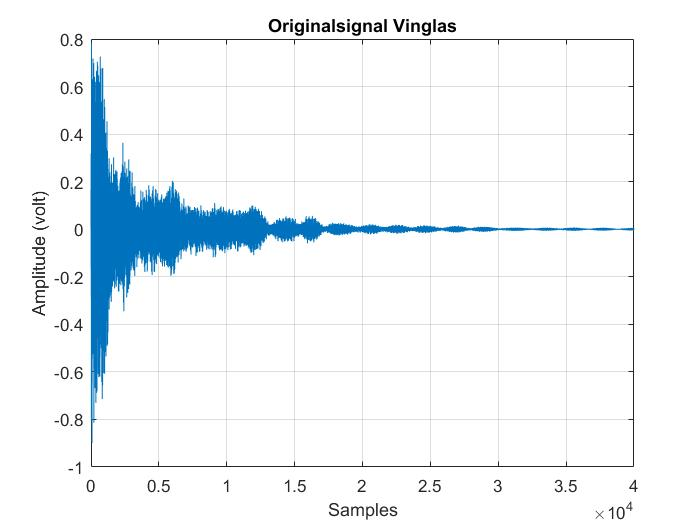
\includegraphics[width=140mm]{figures/Vinglas/original.jpg}
	\caption{DFT Det originale signal fra et Vinglas}
	\label{fig:Vinglas original}
\end{figure}

Det originale signal er blevet fast fourrier transformeret og er blevet plottet på en logoritmisk skala på figur \ref{fig:Vinglas DFT}. Det i øjenfaldende på dette plot er, at det indeholder mange høje frekvenser og har få meget præcise frekvenser, hvor der er stor energi.

\begin{figure}[H]
	\centering
	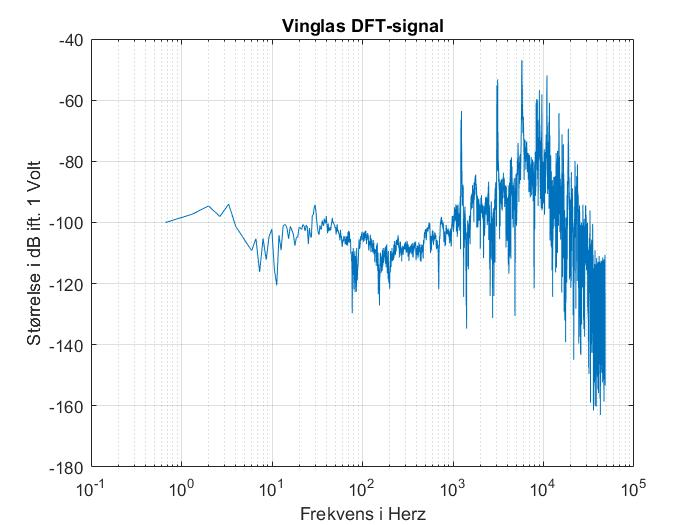
\includegraphics[width=120mm]{figures/Vinglas/DFT.jpg}
	\caption{DFT Analyse af et signal fra et Vinglas}
	\label{fig:Vinglas DFT}
\end{figure}

\begin{figure}[H]
	\centering
	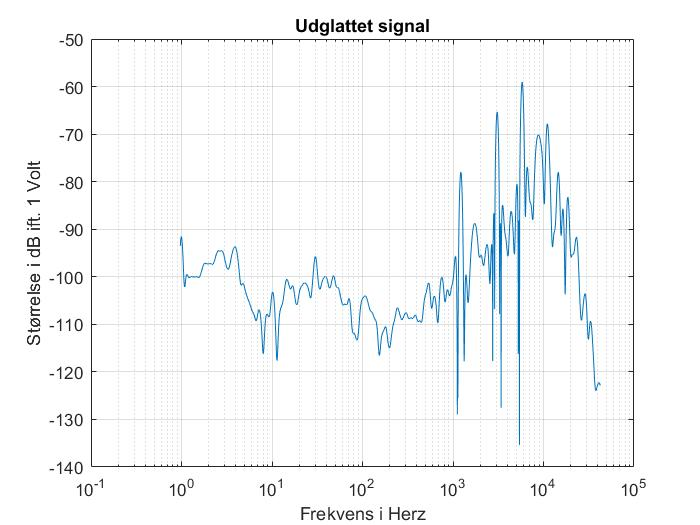
\includegraphics[width=120mm]{figures/Vinglas/udglattet.jpg}
	\caption{Det udglattede DFT signal fra en, der knipser på et vinglas}
	\label{fig:Vinglas udglattet}
\end{figure}



\section{Vindmølle}
Dette signal er larm fra en vindmølle. Man kan se det originale lydsignal på figur \ref{fig:Vinglas original}.
\begin{figure}[H]
	\centering
	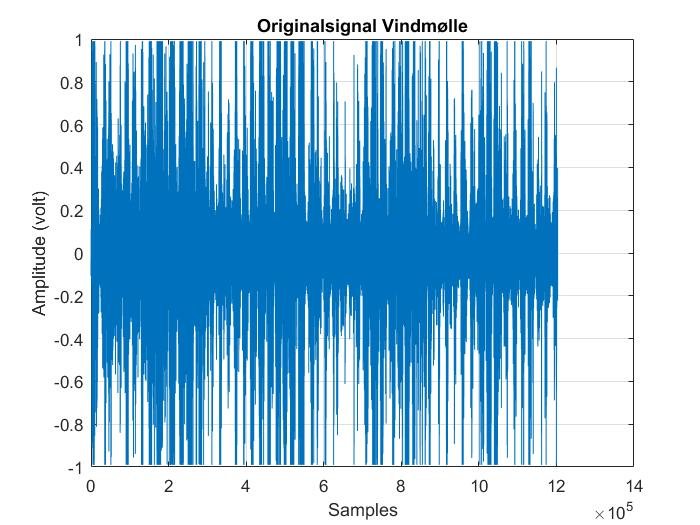
\includegraphics[width=140mm]{figures/Vind/original.jpg}
	\caption{DFT Det originale signal fra en Vindmølle}
	\label{fig:Vind original}
\end{figure}

Det originale signal er blevet fast fourrier transformeret og er blevet plottet på en logoritmisk skala på figur \ref{fig:Vind DFT}. Det i øjenfaldende på dette plot er, det er rimelig lavfrekvent (70Hz-200Hz). Der er heller ikke rigtig specielt mange frekvenser, der stikker specielt ud.
\begin{figure}[H]
	\centering
	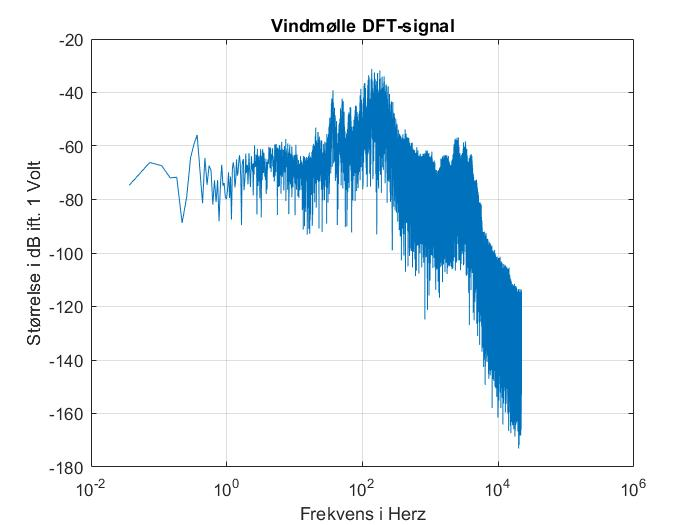
\includegraphics[width=120mm]{figures/Vind/DFT.jpg}
	\caption{DFT Analyse af et signal fra en Vindmølle}
	\label{fig:Vind DFT}
\end{figure}

\begin{figure}[H]
	\centering
	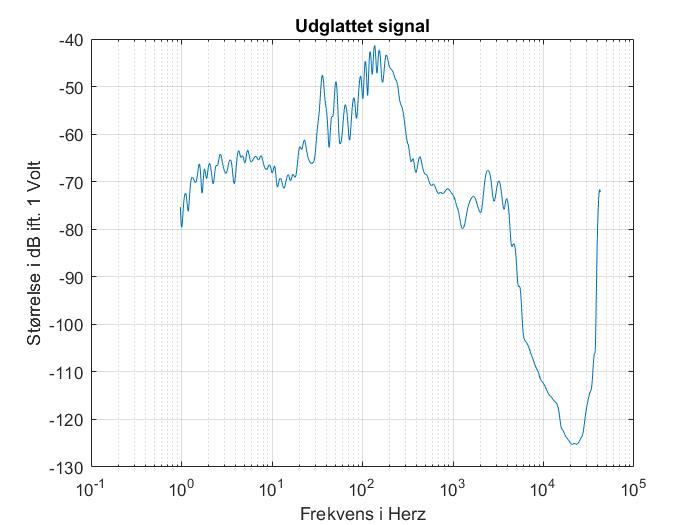
\includegraphics[width=120mm]{figures/Vind/udglattet.jpg}
	\caption{Det udglattede DFT signal fra en Vindmølle}
	\label{fig:Vind udglattet}
\end{figure}


\section{Spilledåse}
Dette signal er musik fra en gammeldags spilledåse. Man kan se det originale lydsignal på figur \ref{fig:Musikbox original}.
\begin{figure}[H]
	\centering
	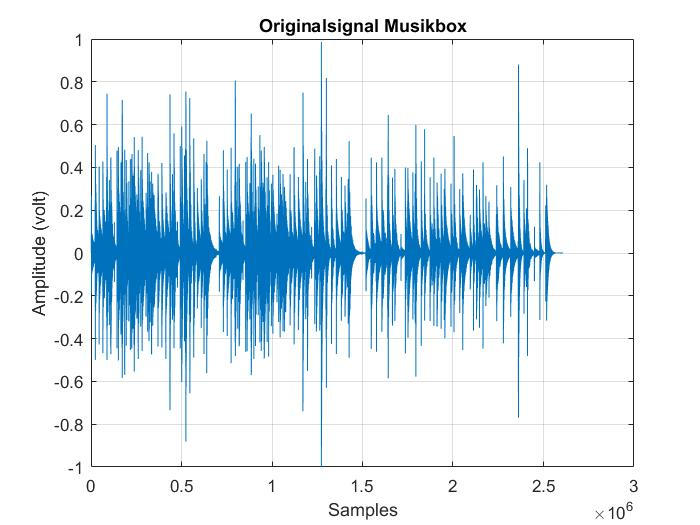
\includegraphics[width=140mm]{figures/Musikbox/original.jpg}
	\caption{Det originale signal fra en Musikbox}
	\label{fig:Musikbox original}
\end{figure}

Det originale signal er blevet fast fourrier transformeret og er blevet plottet på en logoritmisk skala på figur \ref{fig:Musikbox DFT}. Det i øjenfaldende på dette plot er, at det en del frekvenser, der stikker meget ud.
\begin{figure}[H]
	\centering
	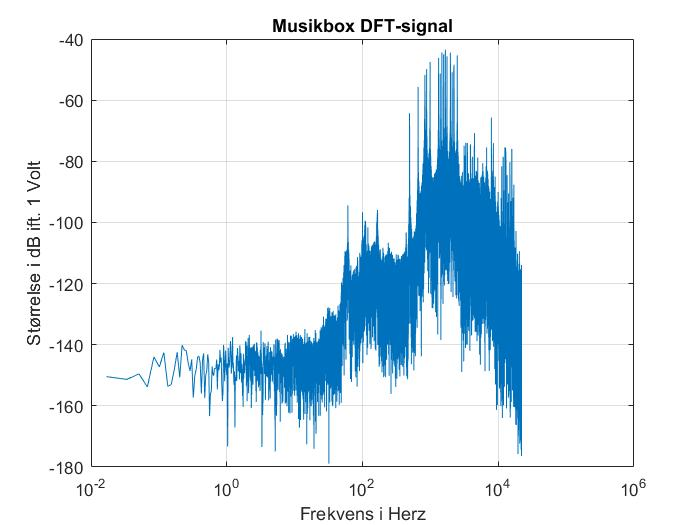
\includegraphics[width=120mm]{figures/Musikbox/DFT.jpg}
	\caption{DFT Analyse af et signal fra en Musikbox}
	\label{fig:Musikbox DFT}
\end{figure}

\begin{figure}[H]
	\centering
	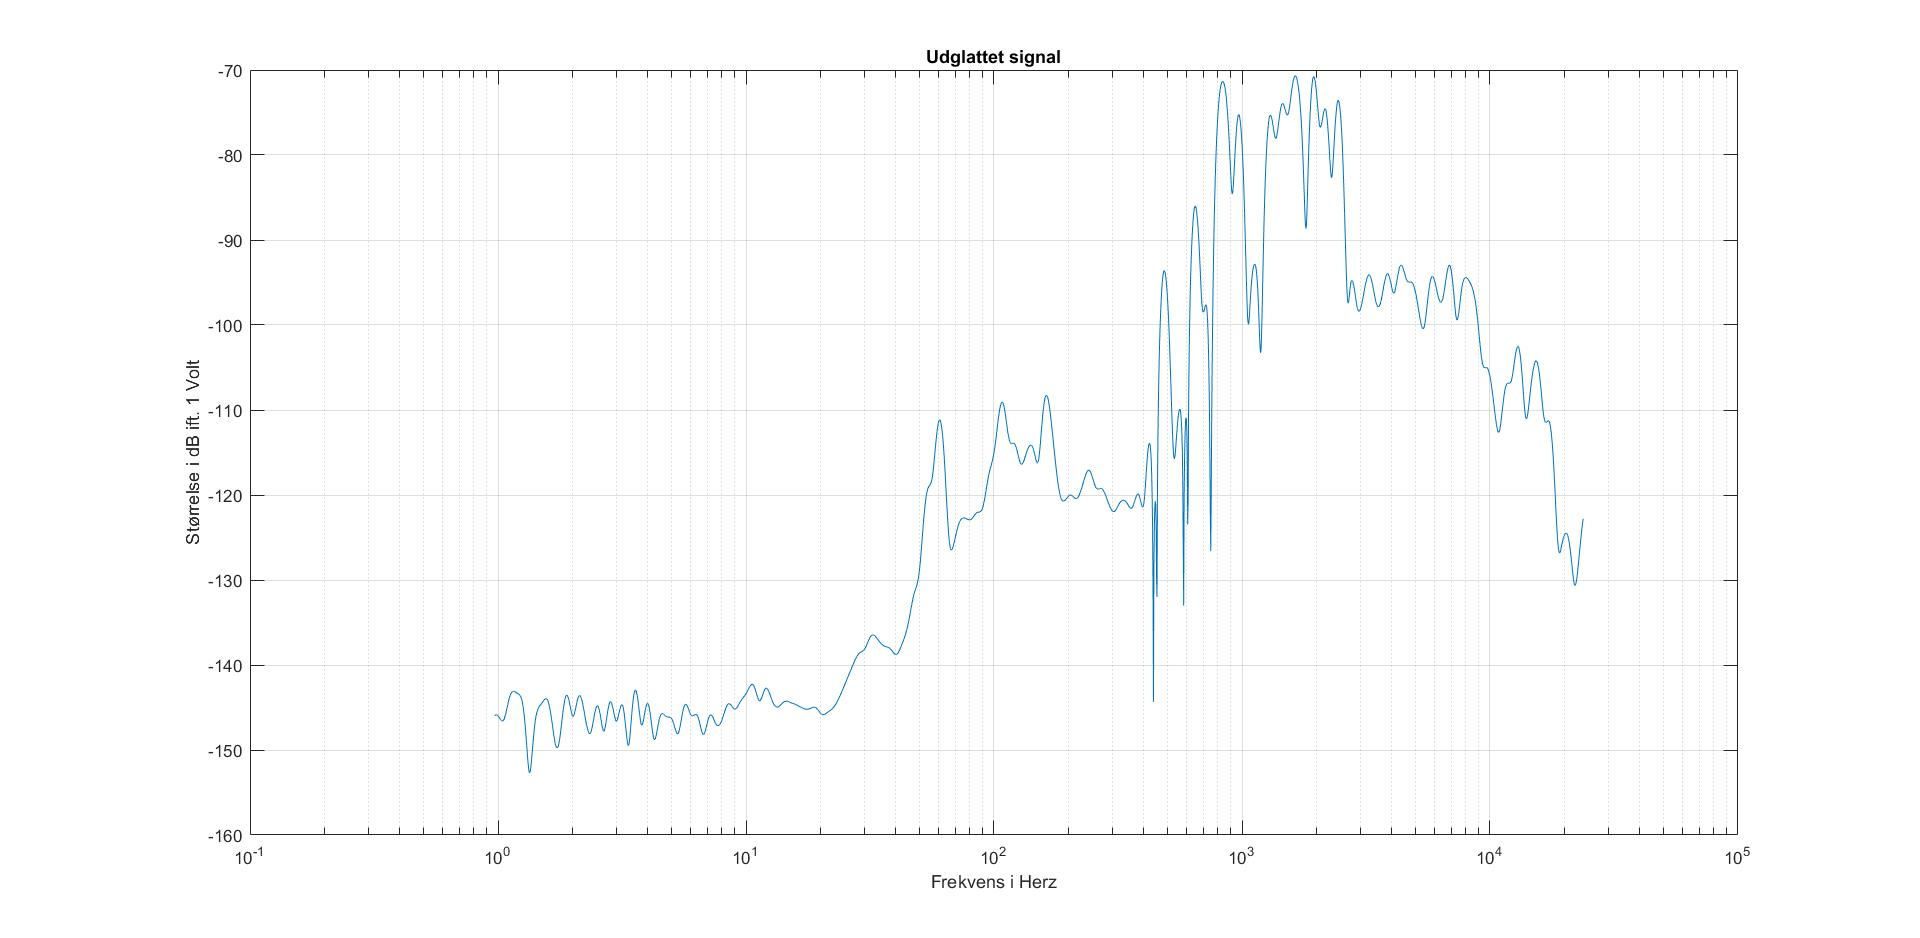
\includegraphics[width=130mm]{figures/Musikbox/udglattet.jpg}
	\caption{Det udglattede DFT signal fra en Musikbox}
	\label{fig:Musikbox udglattet}
\end{figure}
\newpage
\section{ECG-signal}
Dette signal er et ECG-signal. Man kan se det originale lydsignal på figur \ref{fig:ECG original}.
\begin{figure}[H]
	\centering
	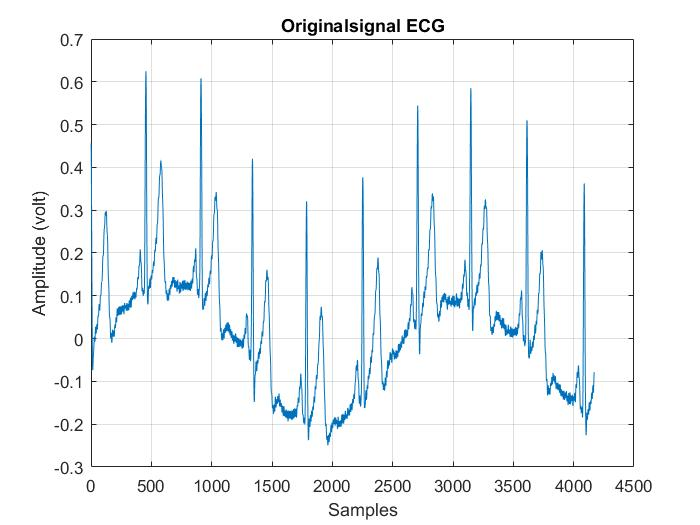
\includegraphics[width=140mm]{figures/ECG/original.jpg}
	\caption{Det originale ECG-signal}
	\label{fig:ECG original}
\end{figure}

Det originale signal er blevet fast fourrier transformeret og er blevet plottet på en logoritmisk skala på figur \ref{fig:ECG DFT}. Det i øjenfaldende på dette plot er, at der meget energi ved de meget lave frekvenser. Man kan også se, at 50Hz stikker voldsomt ud, hvilket er støj fra strømnettet. Dette er meget normalt for ECG-signaler. Generelt har dette signal kun energi udenfor det hørbare frekvensområde. Dette betyder at de fleste mennesker ikke vil kunne høre dette signal.
\begin{figure}[H]
	\centering
	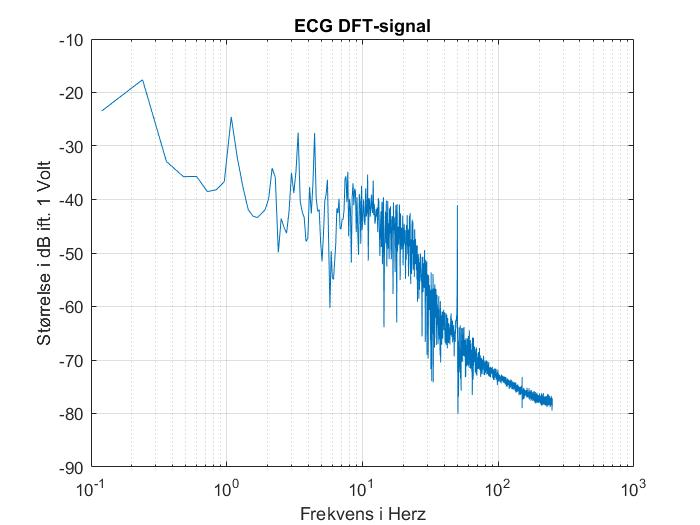
\includegraphics[width=120mm]{figures/ECG/DFT.jpg}
	\caption{DFT Analyse af et ECG-signal}
	\label{fig:ECG DFT}
\end{figure}


\begin{figure}[H]
	\centering
	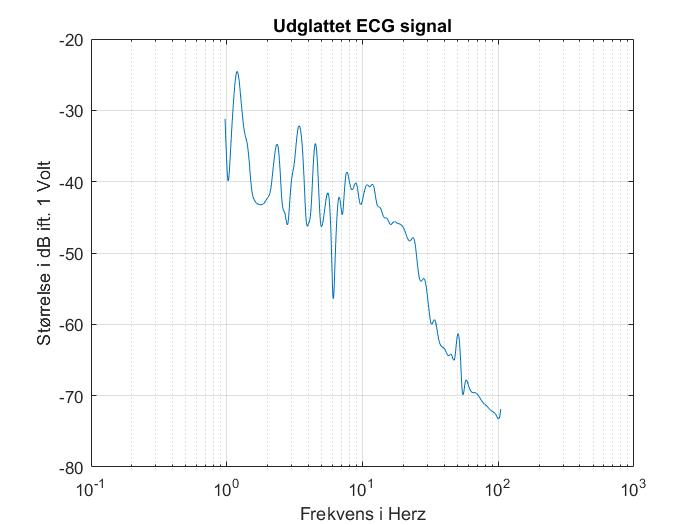
\includegraphics[width=120mm]{figures/ECG/udglattet.jpg}
	\caption{Det udglattede DF140 ECG-signal}
	\label{fig:ECG udglattet}
\end{figure}

